\documentclass{article}
\usepackage{pdfpages}
\usepackage{amsmath}
\usepackage{nicefrac}

\begin{document}

% 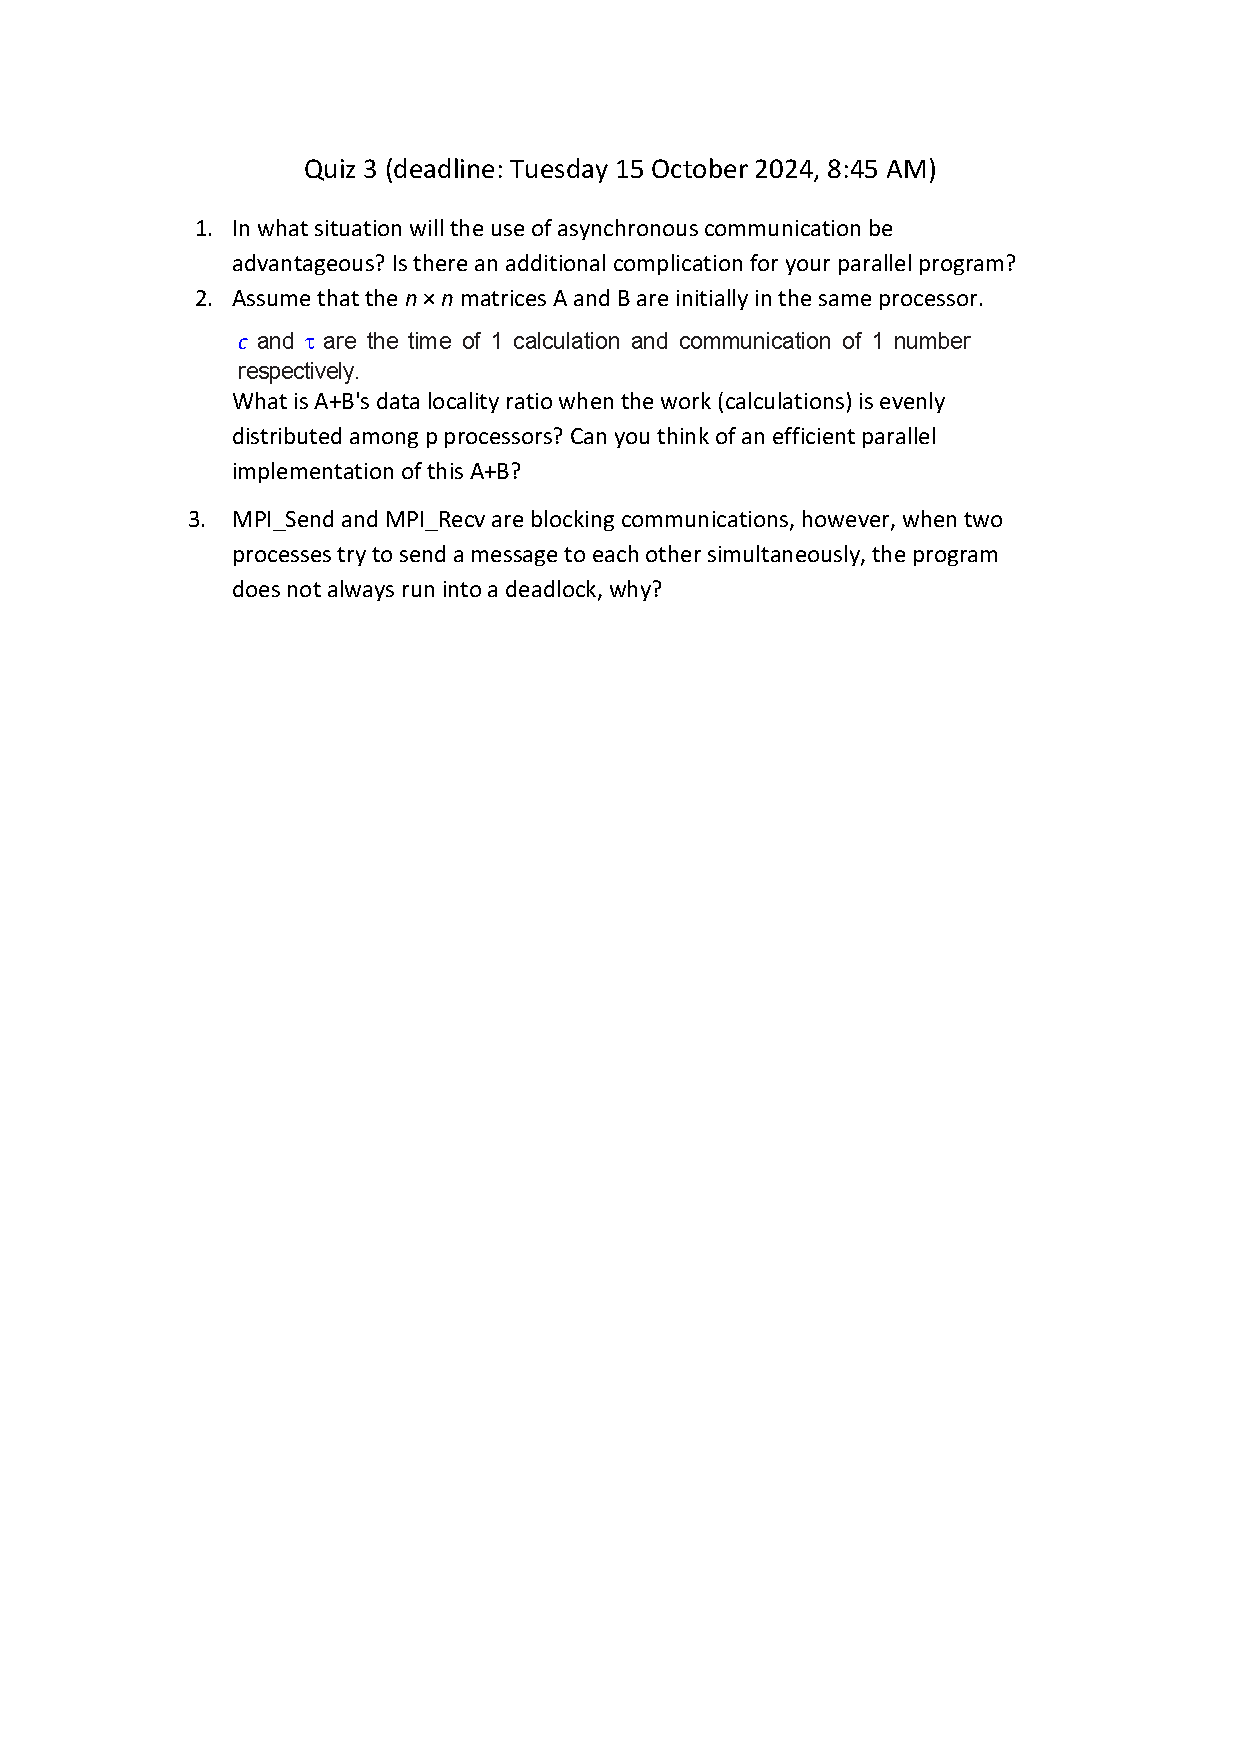
\includepdf[pages={1}]{Quiz 3-2024.pdf}

% Now you can add additional content after the PDF
\huge Quiz 3 - Wachmann Elias (6300421)\\
\normalsize
\vspace{2cm}
\begin{enumerate}
    \item In what situation will the use of asynchronous communication be advantageous? Is there an additional complication for your parallel program?\\

    In situations where the given processor can proceed with other calculations right after the data was send. Say for example in programs with varying workloads per processor, the faster ones can already send their data and start working on the next step without having to wait for slower processors. This leads to a speedup in the overall program. Another situation would be the one, where one processor has to send data to multiple other processors. For this example the sender can perform all non-blocking async calls after another without being blocked by slower other processors. The complications which arise are that the program has to be carefully crafted to not get out of sync. Meaning that some processors might still have to wait for data from others. One must try to avoid race conditions and manage the synchronization of the processors properly. \\
    \item Assume that the $n \times n$ matrices A and B are initially in the same processor. $c$ and $\tau$ are the time of 1 calculation and communication of 1 number respectively. What is A+B's data locality ratio when the work (calculations) is evenly distributed among p processors? Can you think of an efficient parallel implementation of this A+B?\\
    
    Data locality ratio is defined as the ratio of the time spent on calculations $T_{\text{comp}}$ to the time spent on communication $T_{\text{comm}}$: 
    \begin{equation*}
        \frac{T_{\text{comp}}}{T_{\text{comm}}}
    \end{equation*}
    For the computation part we obtain: 
    \begin{equation*}
        T_{\text{comp}} = n^2 \cdot c
    \end{equation*}
    because we have to take the sum of all $n \times n = n^2$ elements. For the communication part one processor which has A and B initially needs to send $\nicefrac{n^2}{p}$ elements to each of the other $p-1$ processors and they all have to send it back eventually. This leads to a total communication time of:
    \begin{equation*}
        T_{\text{comm}} = 2 \cdot (p-1) \cdot \tau \cdot \frac{n^2}{p} = 2 \cdot n^2 \cdot \tau \cdot \frac{p-1}{p}
    \end{equation*}
    All in all we get: 
    \begin{equation*}
        \frac{T_{\text{comp}}}{T_{\text{comm}}} = \frac{n^2 \cdot c}{2 \cdot n^2 \cdot \tau \cdot \frac{p-1}{p}} = \frac{c}{2 \cdot \tau \cdot \frac{p-1}{p}} = \frac{c \cdot p}{2 \cdot \tau \cdot (p-1)} \approx \frac{c}{2\cdot\tau}
    \end{equation*}
    Where the last approximations holds for $p \gg 1$.

    In theory (if the communication times are low / non-existing) a parallel implementation could be benefitial. As discussed in the lecture today in practice the communication times are usually too high to make it worth it. Nevertheless, one could implement the following:
    \begin{enumerate}
        \item Distribute blocks of the matrices A and B to the processors. 
        \item Each processor calculates the sum of the elements of the matrices it has.
        \item Each processor sends the result to the master processor.
        \item The master processor gathers all the results in the resulting matrix.
    \end{enumerate}
    \item \texttt{MPI\_Send} and \texttt{MPI\_Recv} are blocking communications, however, when two processes try to send a message to each other simultaneously, the program does not always run into a deadlock, why?\\
    
    We don't always see a deadlock, because typically the \texttt{MPI} implementation buffers especially smaller messages. This is called \textit{eager} sending. The message is stored in a buffer and the process can continue with other calculations. So in this case \texttt{MPI\_Send} actually only block until the message is stored in the buffer. The actual sending of the message is done asynchronously. This is also the reason why we don't always see a deadlock. For larger messages \texttt{MPI} uses \textit{rendezvous} sending. Here the message is only sent when the receiving process is ready to receive it which will lead to a deadlock because both processes are waiting for the other to receive the message.
\end{enumerate}

\end{document}
